\appendix

\phantomsection
\section*{Appendix}


\begin{itemize}
  \item[] \textbf{\ref{app:hitting_benchmarks} Hitting Benchmark Construction and Implementation Details}
    \begin{itemize}
      \item[] \ref{app:fir_extraction} Extraction of Functional Intermediate Representations
      \item[] \ref{app:mppi_annotation} MPPI-based Demonstration Generation
      \item[] \ref{app:implementation_details} Training and Implementation Details
    \end{itemize}
    
  \item[] \textbf{\ref{app:additional_experimental_results} Additional Experimental Results}
    \begin{itemize}
      \item[] \ref{app:more_real_world_experiments} More Real-World Experiments
      \item[] \ref{app:more_qualitative_results} Additional Qualitative Comparisons
    \end{itemize}
\end{itemize}



\section{Hitting Benchmark Construction and Implementation Details}
\label{app:hitting_benchmarks}
This section provides additional details on the construction of our hitting benchmarks. We first describe the extraction of different functional intermediate representations in Appx.~\ref{app:fir_extraction}, then introduce MPPI-based action-label generation in Appx.~\ref{app:mppi_annotation}. Finally, we summarize the training and implementation details of FORGE and all baselines in Appx.~\ref{app:implementation_details}.

\begin{table}[ht]
\centering
\caption{\textbf{Statistics of Functional Intermediate Representations.}
We report the number of tools, settings, initial poses, samples per pose, and total samples for each representation.}
\label{tab:representation_statistics}
\resizebox{\linewidth}{!}{
\begin{tabular}{lccccc}
\toprule
Representation & \# Tools & \# Settings & \# Initial Poses & \# Samples / Pose & \# Total \\
\midrule
Affordance Image & 7 & 1 & 1 & 1 & 7 \\
Human Video Prompts & 7 & 3 & 5 & 5 & 525 \\
Keypoint Trajectories (Simulation) & 7 & 3 & 30 & 1 & 630 \\
Keypoint Trajectories (Real World) & 6 & 2 & 1 & 20 & 240 \\
\bottomrule
\end{tabular}
}
\end{table}

\label{app:fir_extraction}

\begin{figure}[!h]
    \centering
    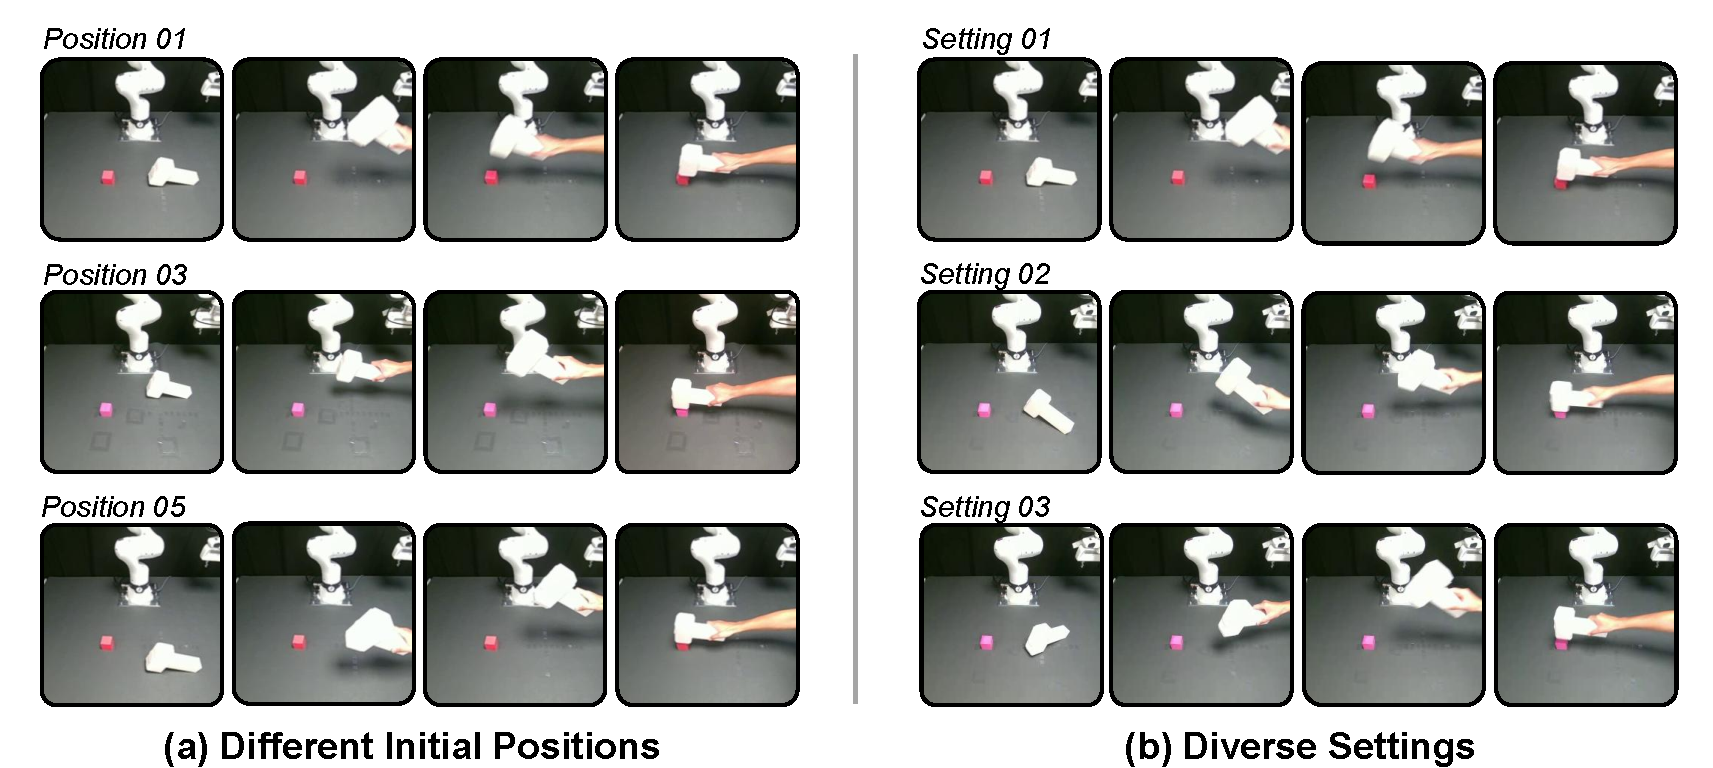
\includegraphics[width=1.0\linewidth]{figures/human-video-prompt.pdf}
    \caption{\textbf{Human Video Prompt Samples.}
    (a) Samples from different initial positions. (b) Samples from different settings.}

    \label{fig:human-video-prompts}
\end{figure}

\subsection{Extraction of Functional Intermediate Representations}
As discussed in Sec.~\ref{sec:Functional Intermediate Representations Selection}, we consider three types of functional intermediate representations: affordance images, human video prompts, and 2D keypoint trajectories. Specifically, we describe how each representation is extracted and incorporated as an additional condition for the grounded execution policy $\pi_{\mathrm{sys1}}$. The statistics of these representations are summarized in Tab.~\ref{tab:representation_statistics}.

\begin{table}[!h]
\centering
\caption{\textbf{Main Reward Terms for MPPI-based Demonstration Generation.}
Here, $d_x$, $d_y$, and $d_{xy}$ denote the distances between the hitting point and the target along the $x$ axis, the $y$ axis, and the $xy$ plane, respectively, while $\Delta d_x$, $\Delta d_y$, and $\Delta d_{xy}$ denote their step-wise reductions.
For the vertical direction, $z_{\mathrm{lift}}$ denotes the tool lifting height from its initial height, $z_1$ denotes the target lifting threshold in Stage~1, $\Delta z_{\mathrm{lift}}$ denotes the step-wise lifting progress, and $e_z$ denotes the error between the current tool height and the target hovering height.
$\Delta z_{\mathrm{head}}$ denotes the vertical displacement of the hitting point between consecutive steps, so $-\Delta z_{\mathrm{head}}$ measures downward motion.
The terms $r_\ast$ reward the current state for satisfying the stage-specific objective, while $r_{\ast\_\mathrm{prog}}$ rewards step-wise progress toward that objective.}

\label{tab:mppi_rewards}
\resizebox{\linewidth}{!}{
\begin{tabular}{lp{0.30\linewidth}p{0.50\linewidth}}
\toprule
Stage & Objective & Main Reward Terms \\
\midrule
Stage 1 
& Lift the tool and align it with the target along the $x$ and $y$ axes.
& 
$
\begin{aligned}
r_{\mathrm{lift}} &= 18.0\min(z_{\mathrm{lift}}, z_1), \\
r_{\mathrm{lift\_prog}} &= 100.0\min(\Delta z_{\mathrm{lift}}, 0.02), \\
r_x &= 22.0\exp(-18.0 d_x), \\
r_{x\_\mathrm{prog}} &= 120.0\min(\Delta d_x, 0.02), \\
r_y &= 8.0\exp(-8.0 d_y), \\
r_{y\_\mathrm{prog}} &= 35.0\min(\Delta d_y, 0.02).
\end{aligned}
$
\\
\midrule
Stage 2 
& Move the tool toward the target while maintaining a suitable hovering height. 
& 
$
\begin{aligned}
r_{xy} &= 14.0\exp(-10.0 d_{xy}), \\
r_x &= 12.0\exp(-18.0 d_x), \\
r_y &= 8.0\exp(-10.0 d_y), \\
r_z &= 7.0\exp(-18.0 e_z), \\
r_{xy\_\mathrm{prog}} &= 95.0\min(\Delta d_{xy}, 0.02), \\
r_{x\_\mathrm{prog}} &= 80.0\min(\Delta d_x, 0.02), \\
r_{y\_\mathrm{prog}} &= 40.0\min(\Delta d_y, 0.02).
\end{aligned}
$
\\
\midrule
Stage 3 
& Finely align the tool-specific hitting point above the target. 
& 
$
\begin{aligned}
r_{xy} &= 14.0\exp(-14.0 d_{xy}), \\
r_x &= 14.0\exp(-24.0 d_x), \\
r_y &= 10.0\exp(-18.0 d_y), \\
r_{xy\_\mathrm{prog}} &= 145.0\min(\Delta d_{xy}, 0.018), \\
r_{x\_\mathrm{prog}} &= 135.0\min(\Delta d_x, 0.018), \\
r_{y\_\mathrm{prog}} &= 110.0\min(\Delta d_y, 0.018), \\
r_z &= 7.0\exp(-18.0 e_z).
\end{aligned}
$
\\
\midrule
Stage 4 
& Keep the hitting point close to the target and execute the downward strike. 
& 
$
\begin{aligned}
r_{xy} &= 12.0\exp(-16.0 d_{xy}), \\
r_x &= 14.0\exp(-28.0 d_x), \\
r_y &= 10.0\exp(-18.0 d_y), \\
r_{xy\_\mathrm{prog}} &= 120.0\min(\Delta d_{xy}, 0.015), \\
r_{x\_\mathrm{prog}} &= 100.0\min(\Delta d_x, 0.015), \\
r_{y\_\mathrm{prog}} &= 80.0\min(\Delta d_y, 0.015), \\
r_{\mathrm{hit}} &= 150.0\min(-\Delta z_{\mathrm{head}}, 0.05),
\end{aligned}
$
\\
\midrule
Contact / Success 
& Encourage valid downward contact with the target.
& 
$
\begin{aligned}
r_{\mathrm{contact}} &= 150.0 \ \text{if valid downward contact}.
\end{aligned}
$
\\
\bottomrule
\end{tabular}
}
\end{table}

\textbf{Affordance Images.}~~ 
We manually annotate the grasp point and hitting region for each tool, producing 7 affordance images. When evaluating functional intermediate representations in Sec.~\ref{sec:Functional Intermediate Representations Selection}, we use the affordance image of the corresponding tool as an additional condition for the grounded execution policy $\pi_{\mathrm{sys1}}$. Since this representation is time-invariant, the same image feature is shared across all time steps of a trajectory.



\textbf{Human Video Prompts.}~~
As shown in Fig.~\ref{fig:human-video-prompts}, we collect human video prompts for all 7 tools. Following the simulation benchmark, each tool has 3 settings. For each setting, we define 5 initial positions and collect 5 videos per position, resulting in 525 human tool-use videos. When evaluating functional intermediate representations, we use the video prompt corresponding to the tool, setting, and sample from Position 01 as an additional condition for the grounded execution policy. These videos provide visual demonstrations of how humans accomplish the same hitting function with different tools. We leave further exploitation of human video prompts, such as learning functional generalization from human tool-use demonstrations, to future work.


\textbf{Keypoint Trajectories.}~~
We adopt 2D keypoint trajectories as the final functional intermediate representation and extract them for both simulation and real-world data. In simulation, the hitting and target points are directly obtained from the simulator. Given the initial hitting point on the tool, we use SAM2~\cite{ravi2025sam} to segment the corresponding tool mask and sample $N=5$ additional tool keypoints with Farthest Point Sampling (FPS), ensuring spatial coverage of the tool geometry. We then track these sampled tool keypoints with CoTracker~\cite{karaev2024cotracker} to obtain their 2D trajectories. Our simulation benchmark contains 7 tools with 3 settings each. For each setting, we randomly initialize 30 hitting and target positions, resulting in 630 simulation samples.
For real-world data, we manually annotate the target and hitting points for each sample and obtain five additional tool keypoints using the same SAM2- and FPS-based procedure. Unlike simulation, where the hitting and target trajectories are available from the simulator, all 7 real-world keypoints are tracked by CoTracker. The real-world benchmark contains 6 tools, each with 2 hitting patterns and 1 initial position. We collect 20 samples for each initial position, resulting in 240 real-world samples.



\subsection{MPPI-based Demonstration Generation}
\label{app:mppi_annotation}

In the simulation benchmark, the action-labeled demonstrations are automatically generated rather than collected through teleoperation. We use a Model Predictive Path Integral (MPPI) planner with a four-stage rollout procedure, whose main reward terms are summarized in Tab.~\ref{tab:mppi_rewards}. The stages sequentially encourage the robot to lift the tool, move it toward the target, align the tool-specific hitting point with the target, and execute the final downward strike.

Besides the translational commands optimized by MPPI, we specify a target rotational pose at the end of each stage and generate the corresponding rotational commands through servo control. This helps the tool maintain an appropriate orientation during lifting, alignment, and hitting. Together, the stage-specific MPPI rewards and rotational servo control enable reliable automatic demonstration generation in simulation.


\begin{figure}[ht]
    \centering
    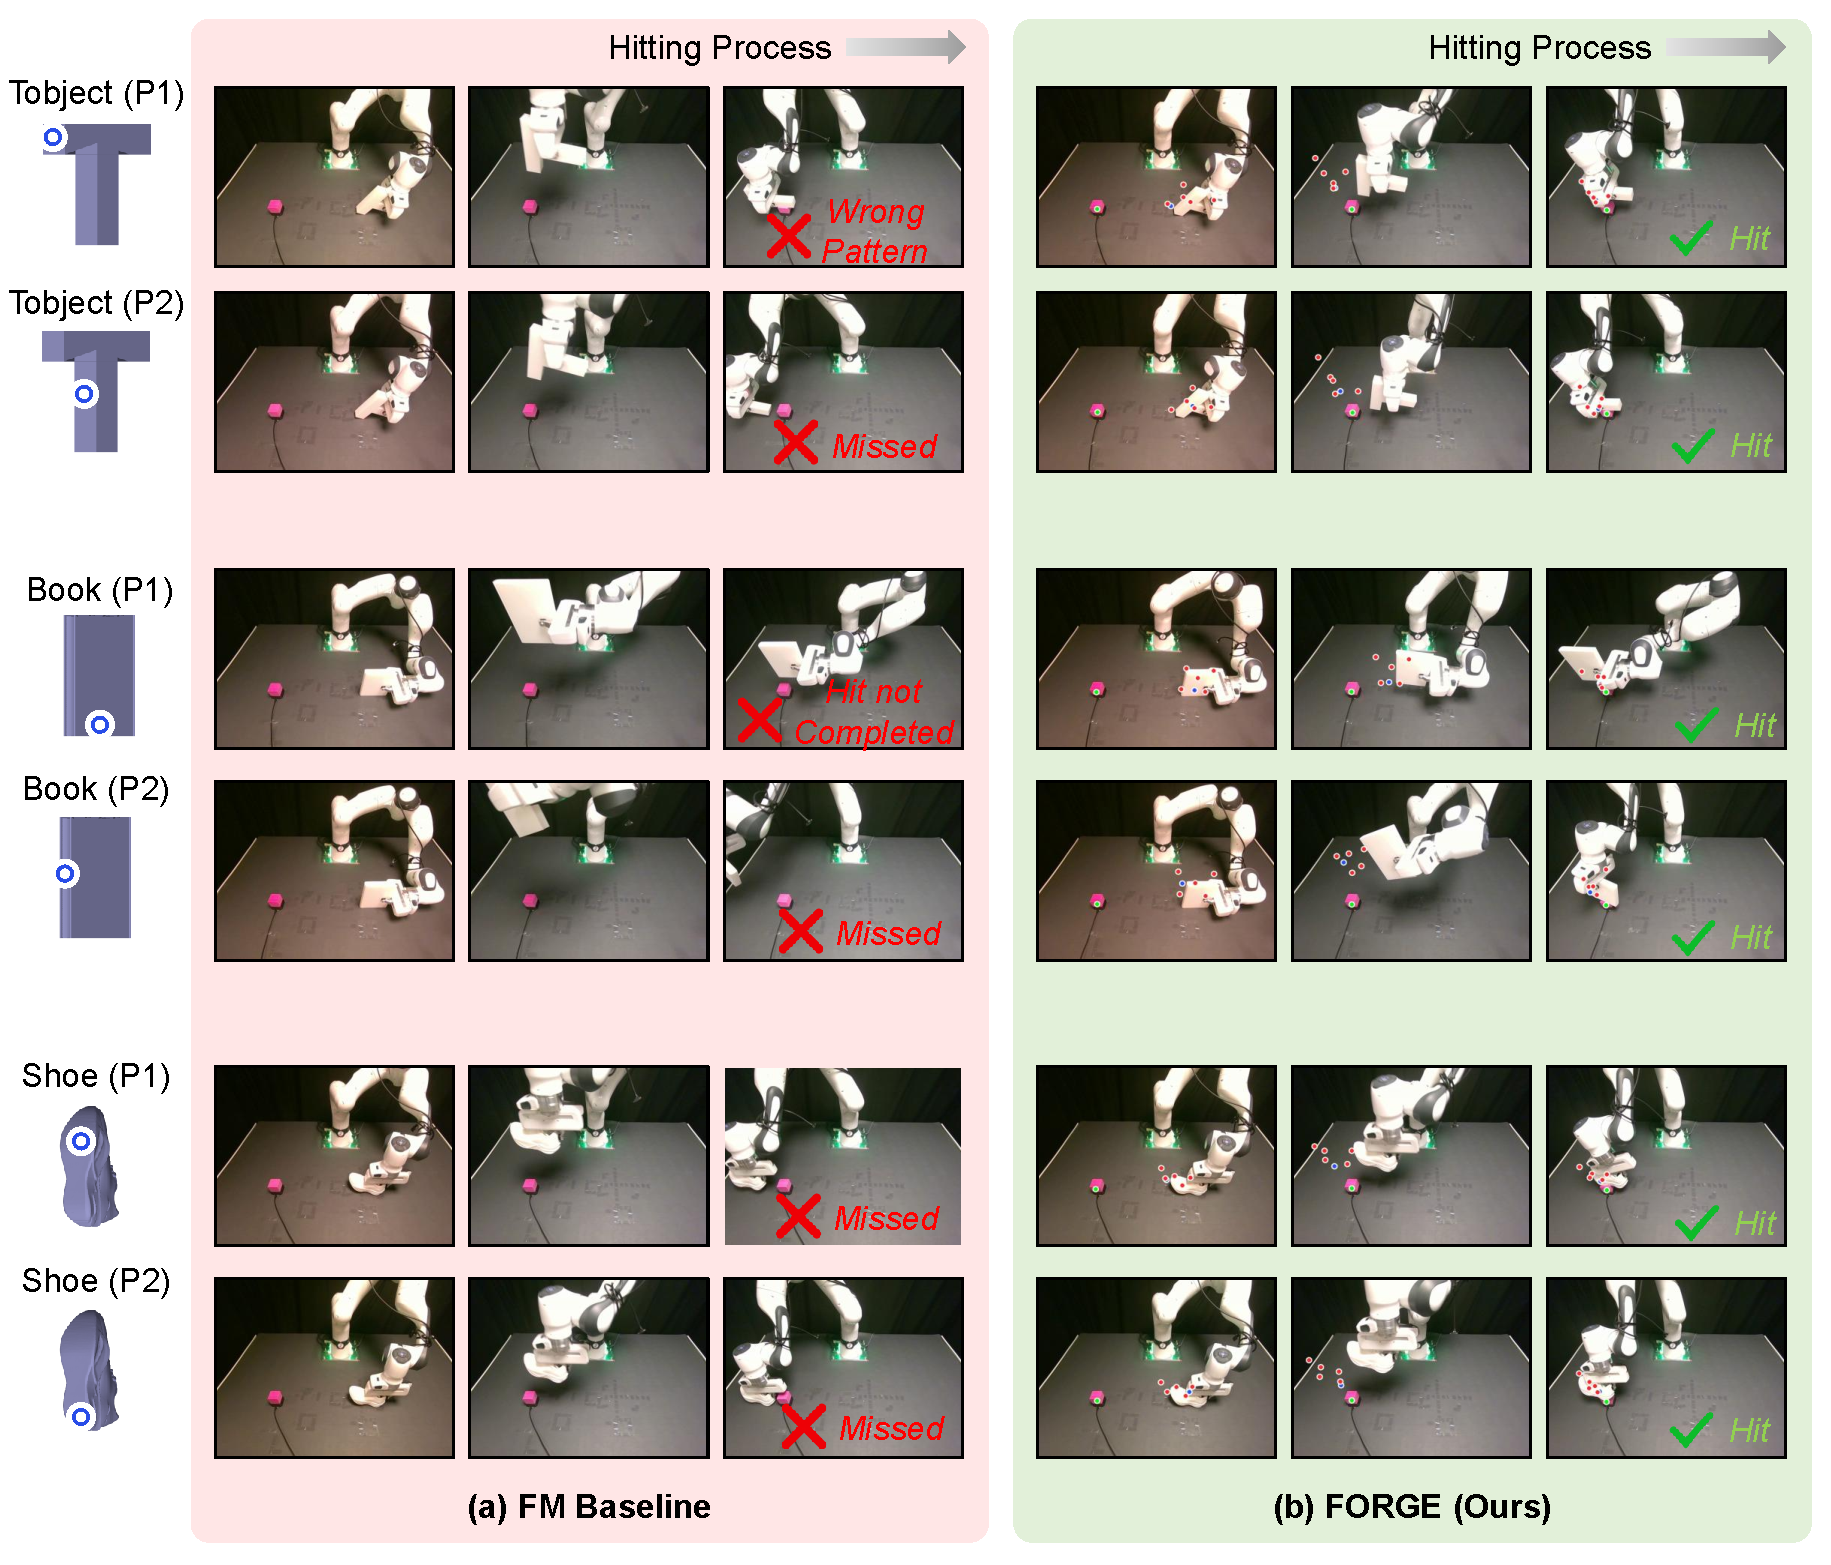
\includegraphics[width=1.0\linewidth]{figures/app-more-real-world.pdf}
    \caption{\textbf{Additional Real-World Qualitative Results.} (a) Failure cases of the FM baseline on unseen tools. (b) Successful demos of \algoname{} across hitting patterns. The blue point indicates the reference hitting point for each pattern.}
    \label{fig:app-more-real-world}
\end{figure}


\subsection{Training and Implementation Details}
\label{app:implementation_details}

All models are trained on NVIDIA RTX 6000 Pro GPUs. For all methods, we use an action chunk size of 8, a history horizon of 8, and a batch size of 64. We build the simulation benchmark on Robomimic and conduct real-world experiments on a Franka robot platform.

For baseline methods, we train each policy for 120,000 steps using the corresponding action-labeled data. For \algoname{}, we follow the two-stage training procedure described in Sec.~\ref{sec:FORGE}. We first pretrain the keypoint motion predictor $\pi_{\mathrm{sys2}}$ on action-free data from all tools for 240,000 steps. We then freeze the pretrained predictor and fine-tune the grounded execution policy $\pi_{\mathrm{sys1}}$ on the same action-labeled data used by the baselines for 120,000 steps.


\begin{table}[ht]
\centering
\caption{\textbf{Additional Real-World Results.}
Success rate (SR) on three unseen tools. Each tool is evaluated under two hitting patterns with 10 rollouts per pattern.}
\label{tab:more_real_world_results}
\resizebox{\linewidth}{!}{
\begin{tabular}{lcccccccccc}
\toprule
\multirow{2}{*}{Method} 
& \multicolumn{3}{c}{Tobject} 
& \multicolumn{3}{c}{Book} 
& \multicolumn{3}{c}{Shoe} 
& \multirow{2}{*}{Overall} \\
\cmidrule(lr){2-4} 
\cmidrule(lr){5-7} 
\cmidrule(lr){8-10}
& P01 & P02 & Avg.
& P01 & P02 & Avg.
& P01 & P02 & Avg.
& \\

\midrule
FM~\cite{lipmanflow} 
& 0.00 & 0.60 & \cellcolor{gray!15} 0.30
& 0.50 & 0.00 & \cellcolor{gray!15} 0.25
& 0.00 & 0.20 & \cellcolor{gray!15} 0.10
& \cellcolor{teal!10} 0.22 \\

\midrule
\algoname{} (Ours) 
& \textbf{0.60} & \textbf{0.80} & \cellcolor{gray!18}\textbf{0.70}
& \textbf{0.60} & \textbf{1.00} & \cellcolor{gray!18}\textbf{0.80}
& \textbf{0.20} & \textbf{0.60} & \cellcolor{gray!18}\textbf{0.40}
& \cellcolor{teal!10}\textbf{0.63} \\
\bottomrule
\end{tabular}
}
\end{table}

\begin{figure}[ht]
    \centering
    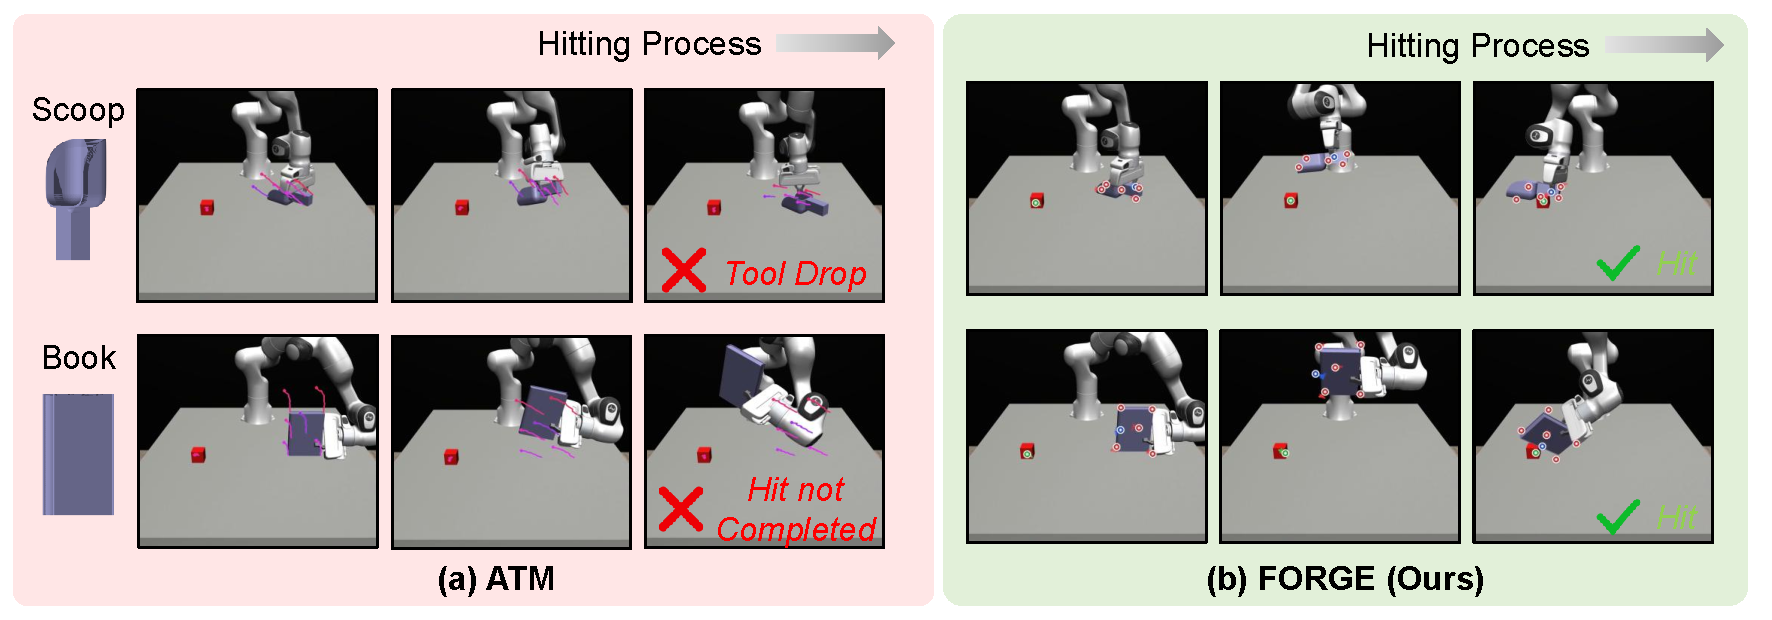
\includegraphics[width=1.0\linewidth]{figures/app-compared-with-ATM.pdf}
    \caption{\textbf{Additional Qualitative Comparison with ATM.}
    (a) Failure cases of ATM on unseen tools. (b) Successful demos of \algoname{} with predicted keypoint-based functional plans.}
    \label{fig:app-compare-atm}
\end{figure}


\section{Additional Experimental Results}
\label{app:additional_experimental_results}

In this section, we first present additional real-world experiments with diverse unseen tools and hitting patterns in Appx.~\ref{app:more_real_world_experiments}, and then provide more qualitative analysis in Appx.~\ref{app:more_qualitative_results}.

\subsection{More Real-World Experiments}
\label{app:more_real_world_experiments}
We conduct additional real-world experiments to evaluate \algoname{} under more diverse tool and hitting-pattern variations. Specifically, we train all methods on three seen tools, including hammer, pickaxe, and mustard, and evaluate them on three unseen tools: tobject, book, and shoe. Each unseen tool contains two hitting patterns, and each pattern is evaluated with 10 real-world rollout trials.

As shown in Tab.~\ref{tab:more_real_world_results}, \algoname{} outperforms the FM baseline across all three unseen tools, improving the overall success rate from 0.22 to 0.63. These results further confirm the main real-world finding: direct perception-to-action mapping struggles to adapt the hitting motion to novel tools, while keypoint-based functional plans provide explicit guidance for aligning the desired hitting region with the target.
The FM baseline mainly fails due to ineffective downward strikes, missed hits, or incorrect hitting patterns. Please refer to our supplementary videos for qualitative demonstrations.

% Please refer to our supplementary videos for qualitative demonstrations.

\subsection{Additional Qualitative Comparisons}
\label{app:more_qualitative_results}

\textbf{More Real-World Cases.}~~
Fig.~\ref{fig:app-more-real-world} provides additional real-world comparisons between the FM baseline and \algoname{} across different unseen tools and hitting patterns. The FM baseline exhibits three typical failure modes: ineffective downward strikes, missed hits, and incorrect hitting patterns. These failures show that an end-to-end policy cannot reliably infer which tool region should be used or how the motion should change for a novel tool. By contrast, \algoname{} uses predicted keypoint-based functional plans to guide contact-region alignment and motion execution, leading to successful hits across these cases. This further supports that functional generalization benefits from an explicit intermediate representation between perception and action. 

\textbf{Comparison with ATM.}~~
Fig.~\ref{fig:app-compare-atm} shows additional qualitative comparisons between ATM and \algoname{} on unseen tools. Although ATM also conditions the policy on keypoint trajectories, these trajectories are produced by a generic tracker and do not explicitly encode function-aware hitting motion. As a result, ATM often fails to guide the tool-specific contact region toward the target, leading to tool dropping or incomplete hits. In contrast, \algoname{} predicts function-aware keypoint trajectories that specify how the hitting point should approach the target before impact, enabling more reliable execution. These results further support our \textbf{H3} in Sec.~\ref{sec:experiments}: keypoint trajectories must encode functional motion intent rather than only generic point tracking.

Please refer to our supplementary videos for demos of both simulation and real-world experiments.



% \begin{table}[t]
% \centering
% \caption{Ablation study on the number of keypoints.}
% \label{tab:ablation_num_keypoints}
% \resizebox{0.5\linewidth}{!}{
% \begin{tabular}{lcccc}
% \toprule
% \# Keypoints & Scoop & Book & Shoe & Avg. \\
% \midrule
% 5 & 0.41 & 0.35 & 0.20 & 0.32 \\
% 7 & 0.42 & 0.42 & 0.23 & 0.36 \\
% 9 & 0.23 & 0.43 & 0.12 & 0.26 \\
% \bottomrule
% \end{tabular}
% }
% \end{table}


% \begin{table}[t]
% \centering
% \caption{\textbf{Ablation on Action-Labeled Tool Diversity.} Success rate (SR) of \algoname{} under different training-to-testing tool splits. `M-to-N' denotes training on $M$ tools and testing on $N$ unseen tools.}
% \resizebox{0.5\linewidth}{!}{
% \begin{tabular}{lcccc}
% \toprule
% Methods & Scoop & Book & Shoe & Avg. \\
% \midrule
% 1-to-3 & 0.17 & 0.10 & 0.14 & 0.14 \\
% 4-to-3 & 0.42 & 0.42 & 0.23 & 0.36 \\
% 7-to-3 & 0.40 & 0.58 & 0.28 & 0.42 \\
% \bottomrule
% \end{tabular}
% }
% \end{table}

% \begin{table}[ht]
% \centering
% \caption{\textbf{Ablation on Action-Labeled Tool Diversity.} Success rate (SR) of \algoname{} under different training-to-testing tool splits. `M-to-N' denotes training on $M$ tools and testing on $N$ unseen tools.}


% \label{tab:ablation_tool_generalization_setting}
% \resizebox{0.9\linewidth}{!}{
% \begin{tabular}{lcccccccc}
% \toprule
% \multirow{2}{*}{Method}
% & \multicolumn{8}{c}{Tools} \\
% \cmidrule(lr){2-9}
% & Hammer & Tobject & Pickaxe & Mustard & Scoop & Shoe & Book & Avg. \\
% \midrule
% \algoname{} (1-to-6) & -- & 0.26 & 0.34 & 0.17 & 0.14 & 0.10 & 0.23 & \cellcolor{teal!10} 0.21 \\
% \algoname{} (4-to-3) & -- & -- & -- & -- & 0.42 & 0.23 & 0.42 & \cellcolor{teal!10} 0.36 \\
% \algoname{} (6-to-1) & -- & -- & -- & -- & -- & -- & 0.52 & \cellcolor{teal!10} 0.52\\
% \bottomrule
% \end{tabular}
% }
% \end{table}

